\textbf{Trefethen 1.4}

Run \texttt{Program 1} to $N = 2^{16}$ instead of $2^{12}$. What happens to the plot of error vs. $N$? Use the MATLAB commands 
\texttt{tic} and \texttt{toc} to generate a plot of approximately how the computation time depends on $N$. Is the dependence
linear, quadratic, or cubic?

\begin{solution}
  At around $10^{-13}$, we find that the error flattens out and machine rounding errors dominate:

  \begin{figure}[h]
    \centering
    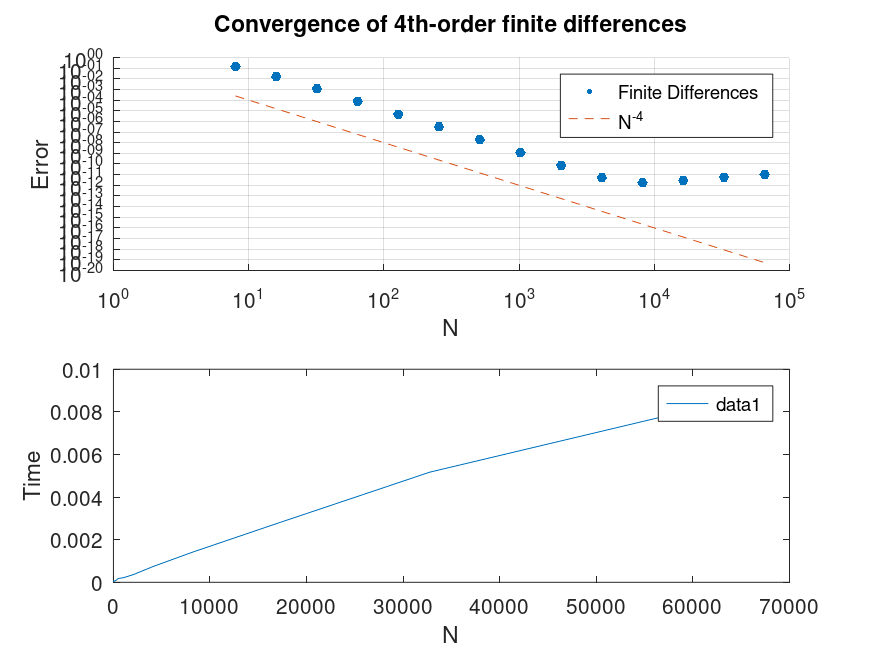
\includegraphics[width=\textwidth]{problem_1_fd.png}
    \caption{Partitions vs. Error and Time}
  \end{figure}

  Moreover, we see that the computation time is approximately linear with respect to the number of equidistant partitions.
  \ \\
\end{solution}